%-*-latex-*-
\sectionthree{Doubly linked list}
\begin{python0}
from solutions import *; clear()
\end{python0}

A doubly linked list is similar to a singly linked list:
For a singly linked list, you start at head
and at every node you can go to the next node (except
when the pointer is NULL).
For a doubly linked list, you can start at the head or tail
and at every node you can go forward and backward.
Here's an example:
\begin{center}
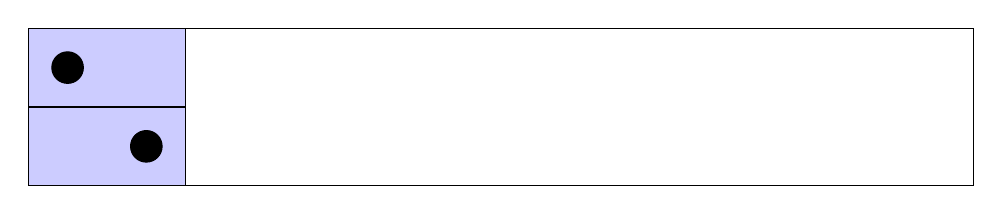
\begin{tikzpicture}

\draw (6.0, 1.0)
  node[draw, , , color=black,
       rounded corners=0cm, inner sep=0cm] {

\begin{minipage}[t][2cm]{12cm}
\mbox{}

\end{minipage}

};
\draw (1.0, 1.5)
  node[fill=blue!20!white,rounded corners=0cm,inner sep=0cm] {

\begin{minipage}[t][1cm]{2cm}
\mbox{}

\end{minipage}

};
\draw (1.0, 1.5)
  node[draw, , , color=black,
       rounded corners=0cm, inner sep=0cm] {

\begin{minipage}[t][1cm]{2cm}
\mbox{}

\end{minipage}

};
\fill[black] (0.5, 1.5) circle (0.2);
\draw[black] (0.5, 1.5) circle (0.2);
\draw (1.0, 0.5)
  node[fill=blue!20!white,rounded corners=0cm,inner sep=0cm] {

\begin{minipage}[t][1cm]{2cm}
\mbox{}

\end{minipage}

};
\draw (1.0, 0.5)
  node[draw, , , color=black,
       rounded corners=0cm, inner sep=0cm] {

\begin{minipage}[t][1cm]{2cm}
\mbox{}

\end{minipage}

};
\fill[black] (1.5, 0.5) circle (0.2);
\draw[black] (1.5, 0.5) circle (0.2);
\end{tikzpicture}

\end{center}



\begin{Verbatim}[frame=single,fontsize=\footnotesize]
class DLNode
{
public:
    DLNode(DLNode * prev = NULL, DLNode * next = NULL)
    : prev_(prev), next_(next)
    {}
    DLNode(int key, DLNode * prev = NULL, DLNode * next = NULL)
    : key_(key), prev_(prev), next_(next)
    {}
private:
    int key_;
    DLNode * prev_;
    DLNode * next_;
};
\end{Verbatim}

The double linked list class would contain two pointers,
one pointing to the head node
and another pointing to the tail node.
If the list is empty, these two pointers are set to NULL.

In the case when the doubly linked list uses
sentinel nodes, you would have
\begin{Verbatim}[frame=single,fontsize=\footnotesize]
class DLList
{
public:
    DLList()
    : pheadsentinel_(new DLNode), ptailsentinel_(new DLNode)
    {
        pheadsentinel_->next_ = ptailsentinel_;
        ptailsentinel_->prev_ = pheadsentinel_;      
    }
private:
    DLNode * pheadsentinel_;
    DLNode * ptailsentinel_;
};
\end{Verbatim}


\newpage
\subsection{Insertion}
Here's insert head:
\begin{Verbatim}[frame=single,fontsize=\footnotesize]
void DLList::insert_head(int v)
{
    DLNode * p = new DLNode(v, pheadsentinel_, pheadsentinel_->next_);
    p->prev_->next_ = p;
    p->next_->prev_ = p;
}
\end{Verbatim}
Note the symmetry in the last two statements -- think of \verb!p! as the
center of attraction so the node before and after \verb!*p! are linked up
with \verb!*p!.
Also, note that it's because of the sentinel nodes that you get
such a clean implementation.
For instance if your doubly-linked class has \verb!phead!
(instead of \verb!pheadsentinel!), you would probably have the following:
\begin{Verbatim}[frame=single,fontsize=\footnotesize]
void DLList::insert_head(int v)
{
    DLNode * p = new DLNode(v, NULL, phead_);
    if (phead_ != NULL)
    {
        phead_->prev_ = p;
    }
    phead_ = p;
}
\end{Verbatim}
For our implementation of the doubly-linked list class, I will be
using sentinel nodes.
I'll leave it to you to write the version without sentinel nodes so that you
see the difference.

There are other ways to implement the above insert head.
Here's another way that is not as simple and symmetric as the above
(and is a lot uglier, in my opinion)
\begin{Verbatim}[frame=single,fontsize=\footnotesize]
void DLList::insert_head(int v)
{
    DLNode * p = new DLNode(v, pheadsentinel_, pheadsentinel_->next_);
    pheadsentinel_->next_ = p;
    p->next_->prev_ = p;
}
\end{Verbatim}
There's also a dependency on \verb!pheadsentinel->next_! in the second
statement.

So what?

Well you might write this:
\begin{Verbatim}[frame=single,fontsize=\footnotesize]
void DLList::insert_head(int v)
{
    DLNode * p = new DLNode(v, pheadsentinel_, pheadsentinel_->next_);
    pheadsentinel->next_->prev_ = p;
    pheadsentinel->next_ = p;
}
\end{Verbatim}
or this:
\begin{Verbatim}[frame=single,fontsize=\footnotesize]
void DLList::insert_head(int v)
{
    DLNode * p = new DLNode(v, pheadsentinel_, pheadsentinel_->next_);
    pheadsentinel->next_ = p;
    pheadsentinel->next_->prev_ = p; // oops 
}
\end{Verbatim}
The second of these two is incorrect. (See it?)

However the second and third statements of the first
insert head can be swapped:
\begin{Verbatim}[frame=single,fontsize=\footnotesize]
void DLList::insert_head(int v)
{
    DLNode * p = new DLNode(v, pheadsentinel_, pheadsentinel_->next_);
    p->prev_->next_ = p;
    p->next_->prev_ = p;
}
\end{Verbatim}

The insert head
\begin{Verbatim}[frame=single,fontsize=\footnotesize]
void DLList::insert_head(int v)
{
    DLNode * p = new DLNode(v, pheadsentinel_, pheadsentinel_->next_);
    p->prev_->next_ = p;
    p->next_->prev_ = p;
}
\end{Verbatim}
can be easily generalized to
\begin{Verbatim}[frame=single,fontsize=\footnotesize]
void DLList::insert_after(DLNode * q, int v)
{
    DLNode * p = new DLNode(v, q, q->next_);
    p->prev_->next_ = p;
    p->next_->prev_ = p;
}
\end{Verbatim}
So in fact \verb!insert_head! can use \verb!insert_after!:
\begin{Verbatim}[frame=single,fontsize=\footnotesize]
void DLList::insert_head(int v)
{
    insert_after(pheadsentinel_, v);
}
\end{Verbatim}
Note that you obviously don't want to insert after the tail sentinel!
So let's prevent that from happening:
\begin{Verbatim}[frame=single,fontsize=\footnotesize]
void DLList::insert_after(DLNode * q, int v)
{
    if (q == psentineltail_)
    {
        throw InsertAfterTailError();
    }
    DLNode * p = new DLNode(v, q, q->next_);
    p->prev_->next_ = p;
    p->next_->prev_ = p;
}
\end{Verbatim}
where \verb!InsertAfterTailError! is some exception class.
Note that the boolean check is redundant if \verb!insert_after!
is never called with \verb!q! $=$ \verb!psentineltail_!.
Linked list classes are meant to work extremely fast.
So like arrays where out-of-bound checks are not executed,
it's also reasonable for a linked list class not to check
if an insert is performed after the tail sentinel.
If so, this should be documented in the linked list class.
%(However see exercise?) 

The mirror image of insert head is
\begin{Verbatim}[frame=single,fontsize=\footnotesize]
void DLList::insert_tail(int v)
{
    DLNode * p = new DLNode(v, ptailsentinel_->prev_, pheadsentinel_);
    p->prev_->next_ = p;
    p->next_->prev_ = p;
}
\end{Verbatim}
See the beauty and the symmetry?

Note that this can be generalized to
\begin{Verbatim}[frame=single,fontsize=\footnotesize]
void DLList::insert_before(DLNode * q, int v)
{
    if (q == pheadsentinel_)
    {
        throw InsertBeforeHeadError();
    }
    DLNode * p = new DLNode(v, q->prev_, q);
    p->prev_->next_ = p;
    p->next_->prev_ = p;
}
\end{Verbatim}
and so
\begin{Verbatim}[frame=single,fontsize=\footnotesize]
void DLList::insert_tail(int v)
{
    insert_before(psentineltail_, v);
}
\end{Verbatim}
But in fact ... note that
\begin{Verbatim}[frame=single,fontsize=\footnotesize]
void DLList::insert_before(DLNode * q, int v)
{
    if (q == pheadsentinel_)
    {
        throw InsertBeforeHeadError();
    }
    insert_after(q->prev_, v);
}
\end{Verbatim}
Nice and beautiful right?



\newpage
\subsection{Deletion}
Now for node deletion:
\begin{Verbatim}[frame=single,fontsize=\footnotesize]
void DLList::delete_at(DLNode * p)
{
    if (p == pheadsentinel_ || p == ptailsentinel_)
    {
        throw DeleteSentinelError();
    }
    p->prev_->next_ = p->next_;
    p->next_->prev_ = p->prev_;
    delete p;
}
\end{Verbatim}
This can then be used for
\begin{Verbatim}[frame=single,fontsize=\footnotesize]
void DLList::delete_head(DLNode * p)
{
    if (is_empty())
    {
        throw UnderflowError();
    }
    else
    {
        delete_at(pheadsentinel_->next_);
    }
}
\end{Verbatim}
and
\begin{Verbatim}[frame=single,fontsize=\footnotesize]
void DLList::delete_tail(DLNode * p)
{
    if (is_empty())
    {
        throw UnderflowError();
    }
    else
    {
        delete_at(ptailsentinel_->prev_);
    }
}
\end{Verbatim}


\newpage
\subsection{Destructor, copy constructor, assignment operator}
Of course with the above methods to acquire resource (memory from the heap),
we need to rewrite
\begin{enumerate}[nosep]
\item the destructor
\item the copy constructor, and
\item the assignment operator
\end{enumerate}

Here's the destructor:
\begin{Verbatim}[frame=single,fontsize=\footnotesize]
DLList::~DLList()
{
    /* The following idea works for singly-linked list:
    DLNode * p = pheadsentinel_;
    while (p != NULL)
    {
        DLNode * q = p->next_;
        delete p;
        p = q;
    }
    */

    DLNode * p = pheadsentinel_;
    while (p != ptailsentinel_)
    {
        p = p->next_;        
        delete p->prev_;
    }
    delete ptailsentinel_;
}
\end{Verbatim}
Can we generalize this?
Yes, for instance we can have a method that removes a \lq\lq section"
of nodes, i.e., a contiguous block of nodes.
I'll call it \verb!DLList::delete(begin, end)! where \verb!begin!
and \verb!end! are addresses and the nodes deleted
are from address \verb!begin! up to \textit{but not including} address \verb!end!.
This can also be used for instance in a method that \textit{clears} the
doubly-linked list so that it becomes empty.
For use by the destructor, since the head and tail sentinels
need not be joined up, I'll have a \verb!delete_! that only
deletes nodes and not join up the two nodes on both ends:
\begin{Verbatim}[frame=single,fontsize=\footnotesize]
void DLList::delete_(DLNode * begin, DLNode * end)
{
    // If necessary, throw an exception if p is pheadsentinel_.
    while (begin != end)
    {
        begin = begin->next_;        
        delete begin->prev_;
    }
}
\end{Verbatim}
Then
\begin{Verbatim}[frame=single,fontsize=\footnotesize]
DLList::~DLList()
{
    delete_(pheadsentinel_, ptailsentinel_);
    delete ptailsentinel_;
}
\end{Verbatim}
\begin{Verbatim}[frame=single,fontsize=\footnotesize]
void DLList::delete(DLNode * begin, DLNode * end)
{
    if (begin != end)
    {
        DLNode * begin_prev = begin->prev_;
        delete_(begin, end);
        begin_prev->next_ = end;
        end->prev_ = begin_prev;
    }
}
\end{Verbatim}
\begin{Verbatim}[frame=single,fontsize=\footnotesize]
void DLList::clear()
{
    delete(pheadsentinel_->next_, ptailsentinel_);
}
\end{Verbatim}


Here's the copy constructor:
\begin{Verbatim}[frame=single,fontsize=\footnotesize]
DLList::DLList(const DLList & list)
    : pheadsentinel_(new DLNode), ptailsentinel_(new DLNode)
{
    pheadsentinel_->next_ = ptailsentinel_;
    ptailsentinel_->prev_ = pheadsentinel_;

    DLNode * p = list.pheadsentinel_->next_;
    while (p != list.ptailsentinel_)
    {
        insert_tail(p->key_);
        p = p->next_;
    }
}
\end{Verbatim}
Note that this uses \verb!insert_tail! so that the new node created
is continually connected to the tail sentinel, which is redundant
except for the tail node.
Here's another version:
\begin{Verbatim}[frame=single,fontsize=\footnotesize]
DLList::DLList(const DLList & list)
    : pheadsentinel_(new DLNode), ptailsentinel_(new DLNode)
{
    DLNode * p = list.pheadsentinel_->next_;
    DLNode * q = pheadsentinel_;
    while (p != list.ptailsentinel_)
    {
        q->next_ = new DLNode(p->key_, q, NULL);
        p = p->next_;
        q = q->next_;
    }
    q->next_ = ptailsentinel_;
    ptailsentinel_->prev_ = q;
}
\end{Verbatim}
Of course the copy constructor is very similar to \verb!operator=!.
\begin{Verbatim}[frame=single,fontsize=\footnotesize]
const DLList & DLList::operator=(const DLList & list)
{
    if (this != &list)
    {
        // 1. Copy key values from list to *this
        // 2. If list has more values, extend *this with values from list
        // 3. If *this has more values, delete extra nodes from *this.
        DLNode * p = list.pheadsentinel_->next_;
        DLNode * q = pheadsentinel_;
        while (p != list.ptailsentinel_ && q != ptailsentinel_)
        {
            q->key_ = p->key_;
            p = p->next_;
            q = q->next_;
        }

        if (p == list.ptailsentinel_)
        {
            delete(q, ptailsentinel_);
        }
        else if (q == ptailsentinel_)
        {
            while (p != list.ptailsentinel_)
            {
                insert_tail(p->key_);
                p = p->next_;
            }
        }
    }
    return (*this);
}
\end{Verbatim}
Note that the last part of the above method
that inserts the values of a section of a list to
a point of another list is helpful.
Here's \verb!insert_after! inserts a sequence of values and not just a single value:
\begin{Verbatim}[frame=single,fontsize=\footnotesize]
DLList::insert_after(DLNode * p, DLNode * begin, DLNode * end)
{
    DLNode * t = p;
    while (begin != end)
    {
        t->next_ = new DLNode(begin->key_, t, NULL);
        t = t->next_;
        begin = begin->next_;
    }
    t->next_ = p->next_;
    p->next_->prev_ = t;
}
\end{Verbatim}
With this,
the copy constructor becomes
\begin{Verbatim}[frame=single,fontsize=\footnotesize]
DLList::DLList(const DLList & list)
    : pheadsentinel_(new DLNode), ptailsentinel_(new DLNode)
{
    insert_after(pheadsentinel_, list.pheadsentinel_->next_, list.ptailsentinel_);
}
\end{Verbatim}
and the \verb!operator=! becomes
\begin{Verbatim}[frame=single,fontsize=\footnotesize]
const DLList & DLList::operator=(const DLList & list)
{
    if (this != &list)
    {
        // 1. Copy key values from list to *this
        // 2. If list has more values, extend *this.
        // 3. If *this has more values, delete part of *this.
        DLNode * p = list.pheadsentinel_->next_;
        DLNode * q = pheadsentinel_;
        while (p != list.ptailsentinel_ && q != ptailsentinel_)
        {
            q->key_ = p->key_;
            p = p->next_;
            q = q->next_;
        }

        if (p == list.ptailsentinel_)
        {
            delete(q, ptailsentinel_);
        }
        else if (q == ptailsentinel_)
        {
            insert_after(ptailsentinel_->prev, p, list.ptailsentinel_);
        }
    }
    return (*this);
}
\end{Verbatim}

Now for search, which is basically linear search.
Note doubly linked lists are \textit{not} really meant for search since the runtime is slow.
\begin{Verbatim}[frame=single,fontsize=\footnotesize]
DLNode * DLList::find(int v)
{
    DLNode * p = pheadsentinel_;
    DLNode * q = list.pheadsentinel_->next_;
    while (q != list.ptailsentinel_)
    {
        p->next_ = new DLNode(q->key_, p, NULL);
        q = q->next_;
        p = p->next_;
    }
    p->next_ = ptailsentinel_;
    ptailsentinel_.prev_ = p;
}
\end{Verbatim}
You can also find in the \lq\lq reverse direction":
\begin{Verbatim}[frame=single,fontsize=\footnotesize]
DLNode * DLList::find(int v)
{
    DLNode * p = ptailsentinel_->next_;
    while (p != pheadsentinel_)
    {
        if (p->key_ == v)
        {
            return p;
        }
        p = p->prev_;
    }
    return NULL;
}
\end{Verbatim}



\begin{ex}
  What will happen if \verb!pheadsentinel_->prev_! is set to
  \verb!pheadsentinel_!? In other words, the previous
  pointer of the head sentinel node is pointing to itself.
  And what will happen if the next pointer of the tail sentinel node
  is pointing to itself?
\end{ex}



\begin{ex}
  Implement the insertion sort on a doubly linked list.
\end{ex}

